\documentclass[answers]{exam}
\usepackage{../../mypackages}
\usepackage{../../macros}


\SolutionEmphasis{\color{blue}}
\renewcommand{\solutiontitle}{\noindent}

%\usepackage{blindtext}

\renewcommand{\arraystretch}{1.5} % Augmente l'espacement vertical entre les lignes du tableau
\newcolumntype{C}{>{\centering\arraybackslash}m{2cm}}


\SetLabelAlign{myright}{\hss\llap{$#1$}}
\newlist{where}{description}{1}
\setlist[where]{labelwidth=2cm,labelsep=1em,
                        leftmargin=!,align=myright,font=\normalfont}

\setlength{\parindent}{0pt}

\title{Devoir sur table N°1}
\author{N. Bancel}
\date{2 Décembre 2024}

\begin{document}


\textbf{Collège Lycée Suger}
\hfill
\textbf{Physique-Chimie} \\

\textbf{Année 2024-2025}
\hfill
\textbf{3ème Cambridge International} \par

{\let\newpage\relax\maketitle}
%\maketitle


  \begin{center}
    \textbf{\textcolor{blue}{Durée du devoir : 1 heure}} \par
    \vspace{1em}
    \textbf{\textcolor{red}{La calculatrice EST autorisée. Total des points : 20 points}} \par
    \vspace{1em}
  \end{center}
  
  \begin{tcolorbox}[colback=gray!10!white, colframe=gray, title=Note importante]
    Toutes les réponses doivent être justifiées : une réponse sans justification est considérée comme fausse. \par
    \vspace{1em}
    Il est permis d'admettre le résultat de certaines questions pour ne pas rester bloqué, en prenant soin d'indiquer sur la copie les résultats admis. \par
    \vspace{1em}
    Des points bonus seront attribués si les résultats sont écrits en notation scientifique (type $a \times 10^n$), ou si la rédaction est particulièrement soignée. \par
    \vspace{1em}
    Barème des points (les exercices peuvent être traités dans le désordre)
    \begin{itemize}[noitemsep]
      \item Exercice 1 : 2.5 points
      \item Exercice 2 : 5 points
      \item Exercice 3 : 4 points
      \item Exercice 4 : 3 points
      \item Exercice 5 : 5.5 points
  \end{itemize}
  \end{tcolorbox}

\section*{Exercice 1 - Les soldats (2.5 points)}

Le prix du plomb ayant fortement augmenté ces dernières années, des escrocs remplacent le plomb utilisé pour fabriquer des figurines par de l'acier (composé majoritairement de fer, moins cher). Les soldats ci-contre sont-ils en plomb ou en acier ?


\begin{tcolorbox}[colback=gray!10!white, colframe=gray, title=Document 1 - Caractéristiques d'un lot de \textbf{25} soldats de plomb]
  \begin{itemize}[noitemsep]
    \item Masse totale : \textbf{1.4 kg}
    \item Volume de métal utilisé par soldat : \textbf{5 $cm^3$}
  \end{itemize}
\end{tcolorbox}

\begin{figure}[H]
  \centering
  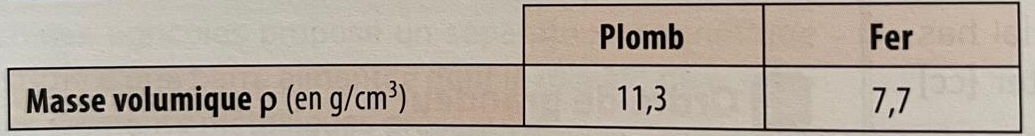
\includegraphics[width=0.8\linewidth]{img/dst_1_01.png}
  \captionsetup{labelformat=empty}
  \caption{\label{} Document 2 - Masse volumique du plomb et du fer}
\end{figure} 


\begin{questions}
  \question[1] Estimer en grammes la masse d'un soldat de plomb.
  \begin{solution}
  
    On commence par calculer la masse d'un soldat en utilisant la masse totale pour 25 soldats.

    \textcolor{blue}{\textbf{Formule utilisée :}}
    \[
    m_{\text{soldat}} = \frac{m_{\text{total}}}{N_{\text{soldats}}}
    \]
    où
    \begin{addmargin}[4em]{1em}
      \begin{compactitem}
          \item [$N_{\text{soldats}}$] représente le nombre de soldats
          \item [$m_{\text{total}}$] représente la masse totale des soldats
          \item [$m_{\text{soldat}}$] représente la  masse d'un soldat
      \end{compactitem}
      \end{addmargin}

  On va vouloir exprimer la masse d'un soldat en grammes, donc on fait d'emblée la conversion nécessaire : $m_{\text{total}} = \SI{1.4}{kg} = \SI{1400}{g}$

  \textbf{Application numérique}
    \begin{align*}
      m_{\text{soldat}} &= \frac{1400}{25} \\
      m_{\text{soldat}} &= 56
    \end{align*}

    \textbf{La masse d'un soldat est donc de 56 g.}
  \end{solution}
  \question[1] Calculer la masse volumique du matériau composant les soldats.
  \begin{solution}
    La masse volumique \( \rho \) est définie par la formule suivante :
    \[
    \rho = \frac{m}{V}
    \]

    Pour un soldat, la masse est \( 56 \ \text{g} \) et le volume est \( 5 \ \text{cm}^3 \). Il suffit d'appliquer la formule du dessus pour déterminer la masse volumique du matériau qui le compose.

    \textbf{Application numérique}
    \begin{align*}
      \rho &= \frac{56}{5} \\
      \rho &= 11.2
    \end{align*}

  \textbf{La masse volumique des soldats est donc de $\SI{11.2}{g/cm^3}$}
  \end{solution}

  \question[0.5] En déduire le matériau utilisé pour fabriquer les soldats.
  \begin{solution}
    \begin{itemize}[noitemsep]
      \item La masse volumique du plomb est \( 11.3 \ \text{g/cm}^3 \).
      \item La masse volumique du fer est \( 7.7 \ \text{g/cm}^3 \).
    \end{itemize}

    \textcolor{blue}{\textbf{La masse volumique mesurée (11.2 g/cm$^3$) est très proche de celle du plomb (11.3 g/cm$^3$). On peut donc en conclure que les soldats sont donc fabriqués en plomb.}} 
  \end{solution}
\end{questions}

\section*{Exercice 2 - L'atome - 5 points}

\begin{questions}
  \question[2] Donner les relations et formules importantes qui font le lien entre le nombre de protons, le nombre d'électrons, le nombre de neutrons, et le nombre de nucléons d'un atome.
  \begin{solution}
    \textcolor{blue}{\textbf{Les relations fondamentales sont :}}
    \begin{itemize}[noitemsep]
      \item Le \textbf{nombre de protons} ($Z$) correspond au \textbf{numéro atomique} de l'\'element.
      \item Le \textbf{nombre de nucl\'eons} ($A$) correspond à la somme du nombre de protons et du nombre de neutrons (que l'on notera $N$) :
      \[
      A = Z + N
      \]
      \item Le \textbf{nombre de neutrons} ($N$) peut donc être déduit par la formule :
      \[
      N = A - Z
      \]
      \item Dans un atome, le \textbf{nombre d'électrons} (que l'on peut noter $N_{e^-}$) est \textbf{égal au nombre de protons} : $N_{e^-} = Z$.
    \end{itemize}

    Ces relations permettent de comprendre la composition d'un atome.
  \end{solution}

  \question[1]  Expliquer pourquoi l'atome est électriquement neutre.

  \begin{solution}
    \textbf{Un atome est \textbf{\'electriquement neutre} car :}
    \begin{itemize}[noitemsep]
      \item Le \textbf{nombre d'électrons} ($e^-$) qui sont chargés \textbf{négativement} est \textbf{égal au nombre de protons} ($Z$) qui sont chargés \textbf{positivement}.
      \item Ainsi, les charges positives des protons compensent exactement les charges négatives des électrons.
    \end{itemize}
    \textbf{Conséquence :} La charge totale de l'atome est nulle (elle vaut $0$).
  \end{solution}

  \question[2] (Extrait du brevet 2023) L'eau de mer contient, au moins en petites quantités, de nombreux éléments chimiques. Parmi ceux-ci, le sodium est présent sous forme d’ion dans le chlorure de sodium. On
donne ci-dessous un extrait de la classification périodique des éléments chimiques qui les
regroupe par ordre croissant de numéro atomique (nombre de protons dans le noyau de
l’élément considéré).

\begin{figure}[H]
  \centering
  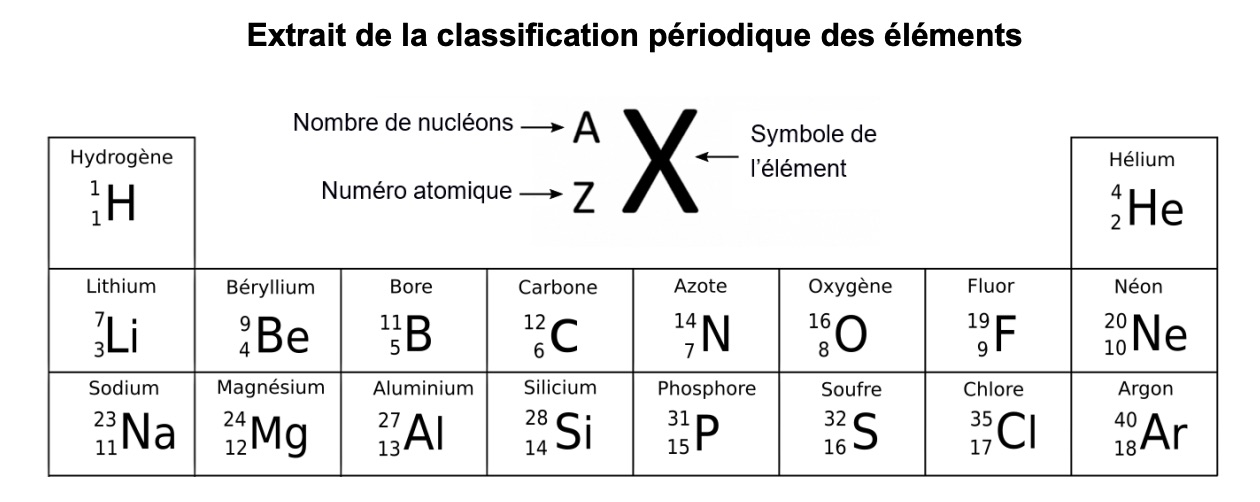
\includegraphics[width=0.8\linewidth]{img/dst_1_02.jpg}
  \captionsetup{labelformat=empty}
  \caption{\label{} Document 3 - Tableau périodique}
\end{figure} 

\begin{parts}
  \part[0.5] Donner le symbole de l'élément sodium 

  \begin{solution}
    \textbf{Le symbole du sodium est \ce{Na}.} \\ 
    Il ne faut pas écrire  $^{23}_{11}\!Na$, ça ne correspondrais pas au SYMBOLE de l'atome Sodium. Ce serait juste retranscrire toutes les informations concernant cet atome (son numéro atomique et son nombre de nucléons). Ici, on ne demande que son symbole.
  \end{solution}
  \part[0.5] Donner le nombre de protons contenus dans le noyau d’un atome de sodium.

  \begin{solution}
    \textbf{Le nombre de protons est égal au numéro atomique ($Z$).}
    Pour le sodium ($\ce{Na}$), $Z = 11$.
    Un atome de sodium contient \textbf{11 protons}.
  \end{solution}

  \part[1] Indiquer le nombre de neutrons contenus dans le noyau d’un atome de sodium. Expliquer la démarche

  \begin{solution}
    \textbf{Formule utilisée :}
    \[
    N = A - Z
    \]
    où $N$ représente le nombre de neutrons, $A$ le nombre de masse (nombre de nucléons) et $Z$ le numéro atomique (nombre de protons)
    \begin{itemize}[noitemsep]
      \item \textbf{Nombre de nucléons} ($A$) pour le sodium : $A = 23$ (donné dans le tableau).
      \item \textbf{Numéro atomique} ($Z$) : $Z = 11$.
    \end{itemize}
    \textbf{Application numérique :}
      \begin{align*}
        N &= 23 - 11 \\
        N &= 12
      \end{align*}
    
    Le noyau d’un atome de sodium contient \textbf{12 neutrons}
  \end{solution}
\end{parts}

\end{questions}

\section*{Exercice 3 - Les incendies - 4 points}

Lors d’un incendie de forêt, les arbres subissent une réaction de combustion. Le bois, assimilé à de
la cellulose de formule chimique simplifiée \ce{C6H10O5}, réagit avec le dioxygène et produit du dioxyde
de carbone et de l’eau à l’état gazeux. L’équation de la réaction est :

\begin{center}
  \ce{C6H10O5 + 6 O2 -> 6 CO2 + 5 H2O}
\end{center}

\begin{questions}
  \question[1.5] L'équation de réaction ci-dessus est-elle équilibrée ? Justifier.

  \begin{solution}
    \textcolor{blue}{\textbf{Pour vérifier si une équation est équilibrée, il faut que le nombre d'atomes de chaque élément soit identique de part et d'autre de l'équation.}}\newline

    \textbf{Étape 1 : Comptons les atomes pour les réactifs (gauche) :}
    \begin{itemize}[noitemsep]
      \item \textbf{Carbone (C)} : 6 atomes dans \ce{C6H10O5}.
      \item \textbf{Hydrogène (H)} : 10 atomes dans \ce{C6H10O5}.
      \item \textbf{Oxygène (O)} :
      \begin{itemize}[noitemsep]
        \item 5 dans \ce{C6H10O5},
        \item 6 dans les 6 molécules de \ce{O2}.
        \item \textbf{Total O réactifs} : 5 + 12 = 17.
      \end{itemize}
    \end{itemize}

    \textbf{Étape 2 : Comptons les atomes pour les produits (droite) :}
    \begin{itemize}[noitemsep]
      \item \textbf{Carbone (C)} : 6 dans les 6 molécules de \ce{CO2}.
      \item \textbf{Hydrogène (H)} : 10 dans les 5 molécules de \ce{H2O}.
      \item \textbf{Oxygène (O)} :
      \begin{itemize}[noitemsep]
        \item 12 dans \ce{CO2} (6x2),
        \item 5 dans \ce{H2O}.
        \item \textbf{Total O produits} : 12 + 5 = 17.
      \end{itemize}
    \end{itemize}

    \textcolor{red}{\textbf{Conclusion : Le nombre d'atomes est identique à gauche et à droite pour chaque élément. L'équation est donc bien équilibrée.}}
  \end{solution}

  \question[1] Lister, \textbf{en Français (et non pas avec la formule scientifique / chimique)}, les réactifs et les produits de cette équation

  \begin{solution}
    \textbf{Réactifs :}
    \begin{itemize}[noitemsep]
      \item Cellulose (bois).
      \item Dioxygène.
    \end{itemize}

    \textbf{Produits :}
    \begin{itemize}[noitemsep]
      \item Dioxyde de carbone.
      \item Eau.
    \end{itemize}
  \end{solution}


  \question[1] On fait réagir du \ce{C6H10O5} et de l'\ce{O2} comme dans la réaction ci-dessus. La masse totale des réactifs est de \SI{39.3}{kg}. Si \SI{10}{kg} de \ce{H2O} sont générés, quelle est la masse de \ce{CO2} produite ? Justifier. 

  \begin{solution}
    \textbf{Principe de conservation de la masse :}
    La masse totale des réactifs est égale à la masse totale des produits :
    \[
    m_{\text{réactifs}} = m_{\text{produits}}
    \]
    On sait aussi que 
\[
  m_{\text{réactifs}} = m_{\ce{C6H10O5}} +  m_{\ce{O2}}
\]
\[
  m_{\text{produits}} = m_{\ce{CO2}} + m_{\ce{H2O}}
\]
On peut donc en déduire que 
\[
  m_{\ce{CO2}} = m_{\text{réactifs}} - m_{\ce{H2O}}
\]

    \textbf{Données :}
    \begin{itemize}[noitemsep]
      \item $m_{\text{réactifs}} = \SI{39.3}{kg}$.
      \item Masse d'eau produite : $m_{\ce{H2O}} = \SI{10}{kg}$.
    \end{itemize}

    \textbf{Application numérique :}
    \begin{itemize}[noitemsep]
      \item Masse totale des produits : $m_{\text{produits}} = m_{\ce{CO2}} + m_{\ce{H2O}}$.
      \item Application numérique :
      \begin{align*}
        39.3 &= m_{\ce{CO2}} + 10 \\
        m_{\ce{CO2}} &= 39.3 - 10 \\
        m_{\ce{CO2}} &= 29.3
      \end{align*}
    \end{itemize}

    \textbf{La masse de \ce{CO2} produite est donc de \SI{29.3}{kg}.}
  \end{solution}

  \question[0.5] (Bonus) A partir de l'équation de réaction, justifier que les incendies produisent des gaz à effet de serre.
  \begin{solution}
    \textbf{Analyse de l'équation :}
    \begin{itemize}[noitemsep]
      \item Lors de la combustion de la cellulose, il y a production de \textbf{dioxyde de carbone} \ce{CO2}.
      \item Le \ce{CO2} est un \textbf{gaz à effet de serre} car il participe au réchauffement climatique en retenant la chaleur dans l'atmosphère.
    \end{itemize}
    \textbf{Conclusion : Les incendies de forêt libèrent des gaz à effet de serre, contribuant au réchauffement climatique.}
  \end{solution}
\end{questions}


\section*{Exercice 4 - Déduction de formules (3 points)}

\begin{tcolorbox}[colback=gray!10!white, colframe=gray, title=Document 4 - La vitesse]
  Contexte : La vitesse d'un objet peut se calculer en mesurant en distance, et en déterminant le temps qu'il a fallu à cet objet pour parcourir cette distance. Sa formule s'écrit
  \[
  v = \frac{d}{t}
  \]
  où 

  \begin{addmargin}[4em]{1em}
    \begin{compactitem}
        \item [v]: représente la vitesse de l'objet
        \item [d]: représente la distance parcourue
        \item [t]: représente le temps écoulé pour que l'objet parcourt la distance
    \end{compactitem}
    \end{addmargin}
  \end{tcolorbox}


\begin{questions}
  \question[1.5] Si dans un problème, je connais la valeur de la vitesse d'un véhicule, et je sais combien de temps il a roulé, comment puis-je déduire la distance qu'il a parcourue ? \textbf{Une réponse sans justification vaudra 0 point}

  \begin{solution}
    Partons de la formule de base :
    \begin{equation}
    v = \frac{d}{t}.
    \end{equation}

    Pour isoler $d$, il suffit de multiplier chaque côté de l'équation par $t$ (ce qui revient à se débarrasser de la division par $t$ dans le membre de droite, et donc d'isoler $d$) :
    \begin{align*}
    v \cdot t &= \frac{d}{\cancel{t}} \cdot \cancel{t} \\
    v \cdot t &= d
    \end{align*}

    Ainsi, on obtient la formule :
    \begin{equation}
    d = v \cdot t.
    \end{equation}

    \textbf{Conclusion :} Si la vitesse ($v$) et la durée ($t$) sont connues, on multiplie simplement $v$ par $t$ pour trouver la distance parcourue ($d$). \par
    \vspace{1em}
    \textbf{ASTUCE : Faites vous un exemple dans votre tête. Vous imaginez que vous connaissez la vitesse de votre voiture : $\SI{130}{km/h}$. Et vous connaissez la durée de votre trajet : vous avez décidé de rouler pendant 2 heures avant de faire une pause. Si je vous demande combien de distance vous aurez parcouru : vous répondrez naturellement $\SI{260}{km}$. Vous venez de faire l'opération $130 \times 2$ et donc de multiplier $v$ par $t$ pour obtenir $d$}
  \end{solution}


  \question[1.5] Si dans un problème, je connais la valeur de la vitesse d'un véhicule, et je sais quelle distance il a parcouru, comment puis-je déduire le temps / la durée pendant laquelle il a roulé ? \textbf{Une réponse sans justification vaudra 0 point}
  \begin{solution}
    Reprenons encore la formule de base :
    \begin{equation}
    v = \frac{d}{t}.
    \end{equation}

    Cette fois, pour isoler $t$, nous devons d'abord inverser la division par $t$. Cela se fait en multipliant chaque côté de l'équation par $t$ :
    \begin{align}
    v \cdot t &= \frac{d \cdot \cancel{t}}{\cancel{t}}, \\
    v \cdot t &= d.
    \end{align}

    Ensuite, pour isoler $t$, il suffit de diviser chaque côté de l'équation par $v$ :
    \begin{align}
    \frac{\cancel{v} \cdot t}{\cancel{v}} &= \frac{d}{v}, \\
    t &= \frac{d}{v}.
    \end{align}

    \textbf{Conclusion :} Si la distance ($d$) et la vitesse ($v$) sont connues, on divise $d$ par $v$ pour trouver la durée ($t$).
  \end{solution}
\end{questions}

\section*{Exercice 5 - Conversions et autres petits exercices (5.5 points)}

\begin{questions}
  \question[2] L'équation suivante est-elle équilibrée ? Justifier. Si elle ne l'est pas, l'équilibrer.
  
  \[
  \ce{N2 + H2 -> NH3}
  \]

  \begin{solution}
    Pour vérifier si une équation est équilibrée, il faut compter le nombre d'atomes de chaque élément de part et d'autre de l'équation.

    \textbf{À gauche :}
    \begin{itemize}
      \item \textbf{Azote (N)} : 2 atomes dans \ce{N2}.
      \item \textbf{Hydrogène (H)} : 2 atomes dans \ce{H2}.
    \end{itemize}

    \textbf{À droite :}
    \begin{itemize}
      \item \textbf{Azote (N)} : 1 atome dans \ce{NH3}.
      \item \textbf{Hydrogène (H)} : 3 atomes dans \ce{NH3}.
    \end{itemize}

    \textbf{Conclusion :} L'équation n'est pas équilibrée car le nombre d'atomes n'est pas identique à gauche et à droite.

    \textbf{Équilibrage :}
    Ajoutons les coefficients nécessaires :
    \[
    \ce{N2 + 3 H2 -> 2 NH3}
    \]

    \textbf{Vérification après équilibrage :}
    \begin{itemize}
      \item \textbf{Azote (N)} : 2 à gauche (\ce{N2}), 2 à droite (2x\ce{NH3}).
      \item \textbf{Hydrogène (H)} : 6 à gauche (3x\ce{H2}), 6 à droite (2x3 dans \ce{NH3}).
    \end{itemize}

    L'équation est maintenant équilibrée.
  \end{solution}
  
  \question[1] Effectuer la conversion suivante : \( 0,0024 \, \mathrm{km} \) à convertir en \textbf{cm}. Justifier.
  \begin{solution}
    \textbf{Formule utilisée :} Pour convertir des kilomètres (km) en centimètres (cm), on utilise les facteurs de conversion suivants :
    \begin{itemize}
      \item \( 1 \, \mathrm{km} = 1000 \, \mathrm{m} \)
      \item \( 1 \, \mathrm{m} = 100 \, \mathrm{cm} \)
    \end{itemize}

    \textbf{Étapes de conversion :}
    \begin{align*}
      0,0024 \, \mathrm{km} &= 0,0024 \times 1000 \, \mathrm{m} \\
      &= 2,4 \, \mathrm{m} \\
      &= 2,4 \times 100 \, \mathrm{cm} \\
      &= 240 \, \mathrm{cm}.
    \end{align*}

    \textbf{Résultat final :} \( 0,0024 \, \mathrm{km} = 240 \, \mathrm{cm} \).
  \end{solution}
  \question[2.5] Un homme pèse \SI{84}{kg} et porte une valise de \SI{21}{kg}. De combien de fois l'homme est-il plus lourd que sa valide ? Justifier (à l'aide d'une formule). A partir des données ci-dessous, déterminer de combien de fois la masse d'un nucléon est plus grande (ou plus petite ?) que celle d'un électron. Pourquoi peut-on dire que la masse d'un atome est pratiquement égale à celle de son noyau.

  \begin{center}
    \begin{tabular}{SS}
      \toprule
      {Constituant} & {Masse (en \si{kg})} \\
      \midrule
      {Electron} & {\(9.1 \times 10^{-31}\)} \\
      {Nucléon (Proton et Neutron)} & {\(1.7 \times 10^{-27}\)} \\
      \bottomrule
    \end{tabular}
  \end{center}
\end{questions}

\begin{solution}
  \textbf{1. Comparaison de la masse de l'homme et de la valise :}
  \begin{itemize}
    \item \textbf{Formule utilisée :} \( \text{Rapport} = \frac{\text{masse de l'homme}}{\text{masse de la valise}} \)
    \item \textbf{Application numérique :}
    \begin{align*}
      \text{Rapport} &= \frac{84}{21} \\
      &= 4.
    \end{align*}
  \end{itemize}
  \textbf{Conclusion :} L'homme est \textbf{4 fois plus lourd} que sa valise. L'idée de cette première partie d'exercice est d'illustrer que ce n'est pas plus compliqué que ça de calculer un rapport de masse ou un rapport de volume. En revanche, je veux que vous POSIEZ L'EQUATION. Cela vous permet de mettre en lumière le fait que l'on pose une division, et permet de généraliser la formule. \par
\vspace{1em}
  \textbf{2. Comparaison de la masse d'un nucléon et de celle d'un électron :}
  \begin{itemize}
    \item \textbf{Formule utilisée :} \( \text{Rapport} = \frac{\text{masse d'un nucléon}}{\text{masse d'un électron}} \)
    \item \textbf{Application numérique :}
    \begin{align*}
      \text{Rapport} &= \frac{1,7 \times 10^{-27}}{9,1 \times 10^{-31}} \\
      &= \frac{1,7}{9,1} \times 10^{4} \\
      &= 1,87 \times 10^{3}.
    \end{align*}
  \end{itemize}
  \textbf{Conclusion :} La masse d'un nucléon est \textbf{environ 1870 fois plus grande} que celle d'un électron. \par
  \vspace{1em}
  \textbf{3. Pourquoi la masse d'un atome est pratiquement égale à celle de son noyau ?}
  \begin{itemize}[noitemsep]
    \item La masse d'un électron est très faible par rapport à celle d'un nucléon (environ 1870 fois plus petite).
    \item La masse d'un atome est donc concentrée dans son noyau, qui contient les protons et les neutrons (nucléons).
  \end{itemize}
  \textbf{Conclusion :} La masse d'un atome est pratiquement égale à celle de son noyau.
\end{solution}

\end{document}
